\documentclass[11pt,a4paper]{ivoa}
\input tthdefs

\title{Group Membership Service}

\ivoagroup{Grid and Web Services}

\author{Brian Major}
\author{Patrick Dowler}
\author{Giuliano Taffoni}
\author{Adrian Damian}
\author{Sara Bertocco}
\author{Marco Molinaro}

\editor{Brian Major}

% \previousversion[????URL????]{????Funny Label????}
\previousversion{This is the first public release}

\begin{document}
\begin{abstract}

The Group Membership Service (GMS) specification describes a service interface for determining whether a user is a member of a group.  Membership information can be used to protect access to proprietary resources.  When an authorization decision is needed (whether to grant or deny access to a proprietary resource), a call to GMS can be made to see if the requesting user is a member of the group assigned to protect the resource in question.  Examples of proprietary resources are wide ranging but include: observation data and metadata and scarce or limited services and infrastructure.  Because this specification details how a single group can protect multiple, potentially distributed, resources, it allows for the representation of teams with common authorization rights.  The members of such teams can span multiple organizations but can be managed within a single service.  In this way, GMS offers an interoperable, flexible, and scalable mechanism for sharing proprietary assets with a potential dynamic set of team members.

\end{abstract}

\section*{Acknowledgments}
For the creation of this document we acknowledge the support of the Canadian Space Agency, the National Research Council Canada, the Italian National Institue of Astrophysics, and the Astronomy ESFRI and Research Infrastructure Cluster (ASTERICS).  ASTERICS is a project supported by the European Commission Framework Programme Horizon 2020 Research and Innovation action under grant agreement n. 653477.

\section*{Conformance-related definitions}

The words ``MUST'', ``SHALL'', ``SHOULD'', ``MAY'', ``RECOMMENDED'', and
``OPTIONAL'' (in upper or lower case) used in this document are to be
interpreted as described in IETF standard RFC2119 \citep{std:RFC2119}.

The \emph{Virtual Observatory (VO)} is a
general term for a collection of federated resources that can be used
to conduct astronomical research, education, and outreach.
The \href{http://www.ivoa.net}{International
Virtual Observatory Alliance (IVOA)} is a global
collaboration of separately funded projects to develop standards and
infrastructure that enable VO applications.


\section{Introduction}

Through standard IVOA protocols, many astronomy data centres and institutes offer users access to datasets through Datalink (Datalink \citep{2015ivoa.spec.0617D}) and SODA (Server-side Operations for Data Access \citep{2017ivoa.spec.0517B}, etc), metadata and catalogs through TAP (\citep{2010ivoa.spec.0327D}), and storage through VOSpace (\citep{2018ivoa.spec.0621G}).  There are also many instances of custom access services to astronomy resources.  In certain cases the information within these services is proprietary -- it is only allowed to be accessed by certain individuals.  Due to the wide variety and inherently institute-specific set of rules that may define how the information is proprietary, it is beneficial to the owners and maintainers of the rules to have a standard way of describing who has access to what resources.  Additionally, the rules describing resource access may be determined by an entity external to the holder of these resources.  To these ends, this document sets out a standard, programmatic, and interoperable method of determining whether a given user is allowed to access a given proprietary resource.

The ideas presented by GMS enable data centres to do authorization checks in an interoperable fashion.  In the context of authorization, interoperability can viewed on two levels:  interoperability amongst the cooperating services \emph{within} a data centre, and interoperability \emph{between} data centres.  Because of the orthogonal nature of authorization, these amount to the same problem.

Interoperability aside, GMS describes a simple, general, maintainable, and scalable approach to performing authorization, and so is a recommended architectural pattern for managing access to proprietary resources.

\subsection{Proprietary resources}

Most facilities have a period of time in which only the Principal Investigator and the associated team has access to observation metadata and data files.  Even without a proprietary period, time is required to verify and validate observations before they can be made public.

Programs create higher level products such as catalogs and images.  On many occasions, they must be accessible to only those who are authorized.

Many organizations have internal, custom services with private or sensitive data.  Similarily, organizations are using TAP to to access relational data that serves only internal or operational purposes and should not be exposed to the general public.

In these ways and others, proprietary resources exist.  For these to be made available to those with authorization, we require a consistent way of performing authorization checks.

\subsection{Role within the VO Architecture}

\begin{figure}
\centering

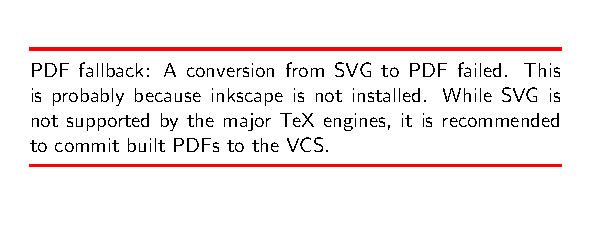
\includegraphics[width=0.9\textwidth]{role_diagram.pdf}
\caption{GMS in relation to the IVOA architecture}
\label{fig:archdiag}
\end{figure}

Fig.~\ref{fig:archdiag} shows the role this document plays within the
IVOA architecture \citep{note:VOARCH}.

GMS can be used by any software that needs to check, for authorization purposes, whether a user is a member of group.  Because of this general purpose functionality, GMS slices through all IVOA standards and lies in the middle of the SHARING technical resource in the IVOA architecture diagram.  Indeed, GMS allows for the sharing of proprietary resources to a limited audience.

\subsection{Use Cases}

Aside from the main use case of restricting access to proprietary resources, GMS supports a number of other use cases, of both the user and system variety.

\paragraph{Proprietary information} Restricting access to proprietary resources to certain users.

\paragraph{Homogeneity} Using the same mechanism to control access to proprietary resources in a data centre or in multiple data centres.

\paragraph{Scalability} A distributed mechanism that scales linearly with the resources being protected.

\paragraph{Remotely managing access} A project may wish to control access to resources that reside externally.

\paragraph{Access rule sharing} A project may consist of a variety of resources that can be all managed by the same access rule: group membership certification.

\paragraph{Extending the services of a data centre} A project that has hosted data and metadata at a data centre may wish to create value-added services outside of the data centre itself.  If some of the data or metadata is proprietary, the extended services may need to determine if a user is allowed to perform certain action on that data or metadata.  A remote GMS instance can be used in this way.

\paragraph{Cooperating institutes} Two or more institutes may work together on a single project that involves proprietary resources and would benefit from a single, standard mechanism for protecting those resources.

\subsection{Definitions}

\paragraph{Authentication} User identification through credentials or identity provider.  Refer to the IVOA Single-Sign-On Profile: Authentication Mechanisms.  \citep{2017ivoa.spec.0524T}

\paragraph{Authorization} Making the decision of whether to grant a user permission to a given resource.  The decision usually involves knowing the user's identity obtained through authentication.

\paragraph{GMS Authorization} Making the decision of whether to grant a user permission to a given resource by ensuring the authenticated user is a member of the group assigned to protect that resource.

\paragraph{Resource} Something that may require authorization for access.  For example, a service, a data file, metadata, a catalog, or infrastructure.

\paragraph{User} An individual or entity identified by authentication that is attempting to perform some action.

\paragraph{Group} A set of users.

\paragraph{Grant} Authorizing access to a proprietary resource by assigning a group to protect that resource.

\paragraph{Revoke} Removing access to a proprietary resource by removing an assigned group.

\paragraph{Owner} A user or group of users who may grant or revoke access to a specific resource.

\section{Authorization Requirements}

When looking at a system that has proprietary resources that need to be protected, it is clear that there are two distinct phases to authorization:  the assignment of the rules protecting the resources, and the attempts by various users to gain access to those resources.  They are described here:

\begin{enumerate}
\item The owner(s) of a resource may, at any time, change the rules by which a resource may be accessed. This is the \emph{granting and revoking of access}.
\item When users try to access resources, the granting rules for that resource are evaluated at runtime. This is the \emph{authorization check}.
\end{enumerate}

With these phases in mind and with the use cases defined, we can state that the goals of authorization are:

\begin{itemize}
\item To allow for restricted access to certain resources: only a certain set of individuals may access certain resources.
\item To allow certain individuals to set the access rules on resources.  The owner(s) of the resources need to manage the access rules.
\item To be able to re-use granting rules between resources.  Projects must authorize access to a variety of proprietary resources.
\item To be able manage granting rules at a single location.  Projects should not have to update each resource on a change to a re-used grant.
\item To be able to reference remote granting rules.  Proprietary resources should not be confined to a single institution.
\end{itemize}

\section{Groups}

\subsection{Why Groups?}

Why are groups a good model for authorization?  When a system needs to perform an \emph{authorization check} on a resource, it is trying to determine if the authenticated user is allowed access.  There are a number of options on how this can be accomplished.

A simple approach would be to add the identity of the user to the resource.  However, this is too restrictive as there may be multiple users who are allowed access.  So, we could instead add a list of user identities to the resource being protected.  It becomes a problem when there are two resources that need protecting by the same set of individuals.  This becomes difficult to maintain because a change in access rules (\emph{granting and revoking access}) would mean a change to multiple resources.

So, it becomes clear that this list of users needs to be decoupled from the resource so that it can be referenced and shared by multiple resources.  To do so, the list must become a single entity than can be referenced by a name.  And so, we must have a named group of users.

A central repository of groups of users would introduce other problems:  a single point of failure, and the inability to partition groups of users.  Thus, the \emph{location} of the group must accompany the group reference so that it is possible to have multiple collections of groups of users and multiple associated GMS services.

Resources must then reference a group by a URI with a location and a name that is unique within that location.  This is called the Group Identifier.

Systems must use the information in the group identifier to determine if the user is a member of the group.  Because the location may be outside of the immediate vicinity of the resource, this query must be performed in a standard and accessible manner and so is defined as a RESTful interface to group membership.

\subsection{Group Identifiers}

A \emph{group identifier} is used to uniquely and universally identify individual groups.  They are attached to proprietary resources for the purpose of referencing the group (or groups) whose members are authorized to access that resource.  When a system needs to do an authorization check because a request for access is being made, it can make the decision based on the response of a membership call to a GMS service.  With the help of an IVOA Registry, the system has all the information it needs within the group identifier to locate the associated GMS service and formulate the REST call to that service for the membership check.

Group identifiers are IVOA Identifiers (IVOIDs) \citep{2016ivoa.spec.0523D}.  This means they can be used to look up the underlying GMS service in an IVOA registry (as is explained in the IVOA Identifiers document).  Group names are specified in the \emph{query} part of the IVOID and are mandatory in group identifiers.  So, group identifiers must conform to all the rules of IVOIDs and also MUST include the \emph{query} part of an IVOID for the group name.

Below is an example of a valid and typical group identifier:

\begin{verbatim}
ivo://authority.example.com/groupService?mygroup
\end{verbatim}

There are two ways to resolve the associated GMS service URL:  lookup the document associated with \emph{ivo://authority.example.com/groupService} in the registry; or, issue a RegTAP (\citep{2014ivoa.spec.1208D}) query for relevant elements of that document.  Here we explain the RegTAP approach.  Following the recommendations in that specification, the query would be done with three necessary constraints in the where clause:
\begin{itemize}
\item{ivoid} - The \emph{registry part} of the group identifier.
\item{standard\_id} - The desired search feature of GMS.
\item{intf\_role} - Always '\emph{std}', to indicate a standard service is being queried for.
\end{itemize}

and one optional constraint, \emph{security\_method\_id}, used to identify how clients can authenticate to the GMS service.  To find a GMS service that does not require authorization, the value of the security\_method\_id constraint would be NULL.  However, since anonymously accessible GMS services are not likely to exist (see section \ref{subsec:infopriv}), the query should either:

\begin{itemize}
\item include a desired security\_method\_id in the where clause, as specified by the IVOA Single-Sign-On Profile \citep{2017ivoa.spec.0524T}, or;
\item omit the constraint and iterate over the resulting rows to choose an appropriate security method.
\end{itemize}

The following query will return a row for each access\_url and security\_method\_id combination.  The ivoid value is calculated by removing the query string from the group identifier.  Since we are looking to perform an \emph{is member} call, we ask for the GMS search capability, identified by the GMS search standardID (see section \ref{subsec:api}).

\begin{verbatim}
    SELECT access_url, security_method_id
    FROM rr.interface
    NATURAL JOIN rr.capability
    NATURAL JOIN rr.resource
    WHERE
      ivoid = 'ivo://authority.example.com/groupService'
      AND standard_id = 'ivo://ivoa.net/std/gms#search-1.0'
      AND intf_role='std'
\end{verbatim}

Note to authors:  The use of security\_method\_id is undergoing changes in RegTAP 1.1 (possible removal).  This document should be updated accordingly upon its acceptance.

This would result in one or more access URLs capable of supporting a GMS search on the group 'groupName' with its corresponding security method support.  For example, it could return three rows with values:

\vspace{3mm}
\hskip-1.0cm
\begin{tabular}{l l}
\textbf{access\_url} & \textbf{security\_method\_id} \\
\hline
https://server.example.com/gms1/search & ivo://ivoa.net/sso\#tls-with-password \\
https://server.example.com/gms2/search & ivo://ivoa.net/sso\#tls-with-certificate \\
https://server.example.com/gms2/search & ivo://ivoa.net/sso\#cookie \\
\hline
\end{tabular}
\vspace{3mm}

The first row identifies a URL to the GMS search capability supporting username and password authentication.  The second and third rows show a URL that supports both client certificate authentication and cookie authentication.  This also implies that membership information about the group 'mygroup' is available from either access URL.

To then perform the group membership query on any of these URLs, the service would formulate a REST call as defined by the GMS Search API.

\section{GMS Search API}

\subsection{API Definition}
\label{subsec:api}

The Group Membership Service defines a RESTful API \citep{fielding00} that allows for the determination of whether a user is a member of a group.  This is the GMS search capability and is identified by the following standardID:

\begin{verbatim}
    ivo://ivoa.net/std/gms#search-1.0
\end{verbatim}

Within this capability, there are two functions and associated endpoints as described in the table below.

\vspace{3mm}
\begin{tabular}{l l}
\textbf{Function} & \textbf{Endpoint} \\
\hline
boolean isMember(Group, User) & GET /search/\{group\} \\
list<Group> getMemberships(User) & GET /search \\
\hline
\end{tabular}
\vspace{3mm}

Where \emph{search} represents the \xmlel{access\_url} from the RegTAP call and \emph{\{group\}} is the groupName part of a Group Identifier.

For a successful HTTP GET to \xmlel{/search/\{group\}}, the service shall respond with HTTP 200 (OK).  If the user is a member of \xmlel{\{group\}}, the service must repeat the name of the group (ending with a newline as a CRLF\footnote{Carriage Return character (ASCII 13) plus a Line Feed character (ASCII 10)}) in the response body in text/plain format.  If the user is not a member of the group, or if the user is not recognized, or if the group is not recognized, the service must return an empty response body.

A successful HTTP GET to \xmlel{/search} shall return HTTP 200 (OK) with a list of the groupNames in which the user is a member in the response body.  The response must again have a Content-Type of \emph {text/plain}.  Each group (even the last) must end with a CRLF.  If the user is not a member of any groups, or if the user is not recognized, the response body must be empty.

It is the authenticated user (the user making the REST call) who is the subject of the of the membership question.  This user's identity is determined by one of the authentication mechanisms described in the IVOA Single-Sign-On Profile.  If the user cannot be identified from the call because they have not authenticated, the service must respond with HTTP 400 (Bad Request).

For an unsuccessful HTTP GET to \xmlel{/search/\{group\}} or \xmlel{/search}, the service must respond with the appropriate HTTP response code.  Some non-200 response codes and the reason for their response are:

\begin{itemize}
\item{400} - Bad request:  If a calling user could not be identitfied from the HTTP request or from the supplied \xmlel{identity} and \xmlel{identityType} parameters.
\item{500} - Internal error:  A service operation failure.
\end{itemize}

For 400 error responses, is recommended that services include, in the response body, textual information about the problem and how clients should change the request for a successful subsequent request.

\subsection {GMS and Credential Delegation}

It is unlikely that users would need to make use of GMS directly unless they would like to ask the service about their group membership for informational purposes.  The main use cases involve systems and services calling GMS for authorization checks.
  Thus, these systems and services need to make the GMS call
This pattern will be in use when the call is being made by a service that supports and implements the IVOA Credential Delegation Protocol \citep{2010ivoa.spec.0218P}.

TBD

\subsection {Search Examples}

\paragraph{Example 1 - Group access to a VOSpace Node}

A user is trying to download a VOSpace file that has the group-read property set to

\begin{verbatim}
ivo://authority.example.com/gms/instance1?my-collaboration
\end{verbatim}

This resolves (though a RegTAP query for the search API) to URL

\begin{verbatim}
https://server.example.com/groupService/search
\end{verbatim}

To authorize the user, the VOSpace service queries the GMS search service using the user's delegated credentials

\begin{verbatim}
HTTP GET to https://server.example.com/gmsService/search/
    my-collaboration
\end{verbatim}

The GMS service identifies the user, consults its group membership information, and returns a response code of 200 with the string \emph{my-collaboration} (followed by CRLF) written to the response body when confirming the user is a member of group 'my-collaboration'.

\begin{verbatim}
my-collaboration
\end{verbatim}

\paragraph{Example 2 - Group access to table data}

A user issues an ADQL query to a table with row-level authorization in a TAP service.  A read-group column defines which group is allowed to read that row.  The first row that is encountered with a non-null read-group has value:

\begin{verbatim}
ivo://authority.example.com/gms/instance1?my-other-collaboration
\end{verbatim}

In anticipation of more rows to follow, and to avoid needing to make multiple calls to GMS, the TAP service asks for all the user's groups when the first protected row is encountered.  This cached group information can be applied to all subsequent rows processed.  In this example, the service does not have the user's delegated credentials so passes the user information (as parameters) in the search call.

\begin{verbatim}
HTTP GET to
https://server.example.com/gmsService/search
\end{verbatim}

The GMS service returns HTTP 200 and all the groups in which user 'myusername' is a member:

\begin{verbatim}
my-collaboration
my-other-collaboration
my-final-collaboration
\end{verbatim}

The TAP service caches this group membership information for the lifetime of the request so that it can be used if necessary when checking other rows.  If a read-group entry with a different \emph{registry part} of the group identifier is encountered, the TAP service must call that GMS service too and add the list of groups to its cache.

\section {Implementation}

\subsection {Implementation Options}

\begin{itemize}
\item Via Grouper (groups in MySQL, users in LDAP) \footnote{https://www.internet2.edu/products-services/trust-identity/grouper/}
\item LDAP only with memberOf plugin (supports groups-of-groups)
\item VOSpace implementation: ContainerNodes = groups, DataNodes = users
\end{itemize}

\subsection{User Identity}

The concept of users and user identity is core to group authorization.  When a system makes a call to a GMS service to determine if the user trying to access the resource is a member of a group, the GMS service needs to identify that user with the users in various groups.

(Author note: add reference or table of user identity types.)

The collection of data centres and astronomy institutes likely have many ways of identifying users.  They could be using external identity providers, they could have a local database of users, or may have a combination of these and other approaches.  This specification does not require such a design.  Instead, it requires simply that users can be uniquely identified within the scope of a GMS service's realm.  If a user identity reaches beyond the scope of a GMS service's realm (such as an X.509 client certificate), then it, too, may be referenced by the service.

\subsection{Information Privacy}
\label{subsec:infopriv}

User and group membership information may be private, so determining who is allowed to make GMS search calls must be considered when implementing a GMS service.  A GMS implementation may insist that GMS search calls must be made by a certain privileged account only.  This is a reasonable approach when the service is only used with a single organization, but would require the distribution of those privileged credentials to any external sites wishing to use it.

Alternatively, a GMS service could have a policy where only the user who is the subject of the membership assertions is allowed to make the GMS search calls.  This approach lends itself well to external interoperability because there need not be any sharing of credentials or trust arrangements between sites -- it is always only the user who makes the service calls, even when they are transitive.  This is the approach recommended in the  IVOA credential delegation protocol \citep{2010ivoa.spec.0218P}.  So, aside from the architectural benefits of employing this pattern, there are some information privacy concerns that are addressed.

\subsection{Groups of Groups}

It may be functionally attractive to support groups within groups.  If this is implemented, then the service must ensure that this representation is reflected by the service API.  For example, if an isMember(g) call is made, and the group 'g' is a group within another group in which the user is a member, then the service must return true.  The fact that the service supports groups within groups is not exposed through the search API, but the API does not prohibit such an implementation.

If one of the contained groups actually exists at another GMS instance, perhaps outside of the organization, then the service must transitively query that service to determine group membership.

\appendix

\section{Changes from Previous Versions}

\subsection{Changes from WD-GMS-1.0-20190506}
\begin{itemize}
\item{General text changes for clarification in abstract and sections 1, 3}
\item{Removed support for identifying the 'target user' of a GMS call with id parameters.  The 'target user' is now always the user making the REST API call to GMS.}
\item{Added new sub-section: GMS and Credential Delegation}
\end{itemize}

\subsection{Changes from WD-GMS-1.0-20190329}
\begin{itemize}
\item{Reverted Group Identifier to be an IVOID}
\item{Corrected, expanded, and clarified the group identifier registry resolution procedure}
\item{Updated bibliography references}
\end{itemize}

\subsection{Changes from WD-GMS-1.0-20181025}
\begin{itemize}
\item{Changed Group identifier URI to be in the format gms://authority/path?group}
\item{Changed names of params user and principal to identity and identityType}
\item{Corrected API definition to always return 200 on succcess}
\item{REST API now described in a table}
\end{itemize}

% these would be subsections "Changes from v. WD-..."
% Use itemize environments.

\bibliography{ivoatex/ivoabib,ivoatex/docrepo}

\end{document}
